
% VLDB template version of 2020-08-03 enhances the ACM template, version 1.7.0:
% https://www.acm.org/publications/proceedings-template
% The ACM Latex guide provides further information about the ACM template

\documentclass[sigconf, nonacm]{acmart}
\usepackage{graphicx}
\usepackage{caption}
\usepackage{subcaption}
\usepackage{adjustbox}
\usepackage{xspace}
% \usepackage[table]{xcolor}
\PassOptionsToPackage{table}{xcolor}
\usepackage[most]{tcolorbox}
\usepackage{enumitem}
\usepackage{fontawesome5}
% in local machine, uncomment following line and run:
%    pdflatex -shell-escape main.tex
% \usepackage[finalizecache,cachedir=minted-cache]{minted}
% In arXiv, include the minted-cache folder in the submission,
%  uncomment following line and run:
\usepackage[frozencache,cachedir=minted-cache]{minted} % for arXiv
% \usepackage{amssymb}
% \usepackage{amsthm}
% \usepackage{amsmath}
% \usepackage{bbm}
% \usepackage{dsfont}
% \usepackage{xcolor}
% \usepackage{hyperref}
% \usepackage{enumitem}
% \usepackage{xspace}

%% The following content must be adapted for the final version
% paper-specific
\newcommand\vldbdoi{XX.XX/XXX.XX}
\newcommand\vldbpages{XXX-XXX}
% issue-specific
\newcommand\vldbvolume{14}
\newcommand\vldbissue{1}
\newcommand\vldbyear{2020}
% should be fine as it is
\newcommand\vldbauthors{\authors}
\newcommand\vldbtitle{\shorttitle} 
% leave empty if no availability url should be set
\newcommand\vldbavailabilityurl{https://github.com/VIDA-NYU/bdikit-beaker}
% whether page numbers should be shown or not, use 'plain' for review versions, 'empty' for camera ready
\newcommand\vldbpagestyle{plain}

\newcommand{\thought}[1]{{\color[rgb]{0.2,0.39,0.66}(#1)}}
\newcommand{\todo}[1]{{\color[rgb]{1.0,0.0,0.0}(#1)}}
\newcommand{\hsh}[1]{{\color{green!50!black} Henrik: #1}}
\newcommand{\st}[1]{{\color{red!50!black} Sebastian: #1}}

\newcommand{\ulm}[1]{_{\scaleto{\mathrm{#1}}{3pt}}}
\newcommand\at[2]{\left.#1\right|_{#2}}











\newtheorem{assumption}{Assumption}

\DeclareMathOperator*{\argmax}{arg\,max}
\DeclareMathOperator*{\argmin}{arg\,min}

\newcommand{\swname}[1]{\texttt{#1}}
\newcommand{\ie}{i\/.\/e\/.,\/~}
\newcommand{\eg}{e\/.\/g\/.,\/~}
\newcommand{\cf}{cf\/.\/~}

\newcommand{\fig}{Fig\/.\/~}
\newcommand{\defn}{Def\/.\/~}
\newcommand{\sect}{Sec\/.\/~}
\newcommand{\tabl}{Tab\/.\/~}
\newcommand{\algo}{Algorithm~}
\newcommand{\theo}{Theorem~}

\newcommand{\bnnl}{3 hidden layers}
\newcommand{\bnnn}{50 neurons}
\newcommand{\bnna}{tanh activations}

\newcommand{\capt}[1]{\mdseries{\emph{#1}}}

\newcommand{\videolink}{at \url{https://youtu.be/_d7AqTRjz6g}}
\newcommand{\codelink}{\url{https://github.com/wheelbot/mini-wheelbot}}

\newcommand{\fakepar}[1]{\vspace{0mm}\noindent\textbf{#1.}}

\newcommand{\needref}{\textcolor{red}{[REF]}}

\newcommand{\plotfontsize}{9pt}



\begin{document}

% \title{Interactive Data Harmonization with LLM Agents [Vision]}
\title{Interactive Data Harmonization with LLM Agents}

\author{Aécio Santos}
\affiliation{%
	\institution{New York University}
	\city{}
	\state{}
}
\email{aecio.santos@nyu.edu}

\author{Eduardo H. M. Pena}
\affiliation{%
	\institution{Federal University of Technology - Paran\'{a}}
	\city{}
	\state{}
}
\email{eduardopena@utfpr.edu.br}
\authornote{Work done as a visiting researcher at New York University.}


\author{Roque Lopez}
\affiliation{%
	\institution{New York University}
	\city{}
	\state{}
}
\email{rlopez@nyu.edu}

\author{Juliana Freire}
\affiliation{%
	\institution{New York University}
	\city{}
	\state{}
}
\email{juliana.freire@nyu.edu}





\newcommand{\systemname}{\texttt{Harmonia}\xspace}


\begin{abstract}
% Data harmonization is essential for integrating datasets from diverse sources, yet it remains a time-consuming and challenging task due to schema mismatches, varying terminologies, and differences in data collection methodologies.
% This paper outlines our vision for agentic data harmonization systems and introduces \systemname, a novel system that embodies this vision. 
% To automate the synthesis of data harmonization pipelines, our approach combines LLM-based reasoning with a library of established and efficient data integration algorithms that address common data integration challenges. Together with domain experts, these components enable the interactive development of data harmonization pipelines that can be later reused to recreate harmonized datasets.
% We demonstrate \systemname's application in a real-world scenario involving clinical data integration and mapping datasets to standardized vocabularies. % like the Genomic Data Commons (GDC). 
% Finally, we outline open problems, including the need for expert-in-the-loop workflows, the variability of LLM outputs, and reproducibility concerns.
Data harmonization is an essential task that entails integrating datasets from diverse sources. Despite years of research in this area, it remains a time-consuming and challenging task due to schema mismatches, varying terminologies, and differences in data collection methodologies. This paper presents the case for agentic data harmonization as a means to both empower experts to harmonize their data and to streamline the process. We introduce \systemname, a system that combines LLM-based reasoning, an interactive user interface, and a library of data harmonization primitives to automate the synthesis of data harmonization pipelines. We demonstrate \systemname in a clinical data harmonization scenario, where it helps to interactively create reusable pipelines that map datasets to a standard format.
Finally, we discuss challenges and open problems, and suggest research directions for advancing 
our vision. 
% \vspace{-0.5em}
\end{abstract}

\maketitle

% \vspace{-.25em}
% %%% do not modify the following VLDB block %%
% %%% VLDB block start %%%
% \pagestyle{\vldbpagestyle}
% \begingroup\small\noindent\raggedright\textbf{PVLDB Reference Format:}\\
% \vldbauthors. \vldbtitle. PVLDB, \vldbvolume(\vldbissue): \vldbpages, \vldbyear.\\
% \href{https://doi.org/\vldbdoi}{doi:\vldbdoi}
% \endgroup
% \begingroup
% \renewcommand\thefootnote{}\footnote{\noindent
% This work is licensed under the Creative Commons BY-NC-ND 4.0 International License. Visit \url{https://creativecommons.org/licenses/by-nc-nd/4.0/} to view a copy of this license. For any use beyond those covered by this license, obtain permission by emailing \href{mailto:info@vldb.org}{info@vldb.org}. Copyright is held by the owner/author(s). Publication rights licensed to the VLDB Endowment. \\
% \raggedright Proceedings of the VLDB Endowment, Vol. \vldbvolume, No. \vldbissue\ %
% ISSN 2150-8097. \\
% \href{https://doi.org/\vldbdoi}{doi:\vldbdoi} \\
% }\addtocounter{footnote}{-1}\endgroup
% %%% VLDB block end %%%

% %%% do not modify the following VLDB block %%
% %%% VLDB block start %%%
% \ifdefempty{\vldbavailabilityurl}{}{
% \vspace{.15cm} %0.3cm
% \begingroup\small\noindent\raggedright\textbf{PVLDB Artifact Availability:}\\
% The source code, data, and/or other artifacts have been made available at \url{\vldbavailabilityurl}.
% \endgroup
% }
% %%% VLDB block end %%%

% \vspace{-.25em}
\vspace{2.0em}
%---------------------

\section{Introduction}
\label{sec:intro}
% Image editing methods in diffusion models depend on user-defined control directions - users can unlock their creativity using these methods by specifying the desired manipulation through prompts~\cite{gandikota2023concept}, reference images~\cite{ruiz2022dreambooth, kumari2022customdiffusion, gal2022image, chen2024trainingfreeregionalpromptingdiffusion}, or attribute vectors~\cite{parmar2023zero,hertz2022prompt}. In this work, we ask a fundamentally different question: \emph{Can we automatically discover the underlying visual structure of a concept within diffusion model's knowledge?} %Rather than requiring user-specified controls, we aim to decompose the model's internal knowledge into meaningful directions.

% This question touches on a fundamental limitation in how we interact with diffusion models. Current control methods ~\cite{zhang2023addingconditionalcontroltexttoimage, gandikota2023concept, ye2023ipadaptertextcompatibleimage,ye2023ipadaptertextcompatibleimage, hertz2024stylealignedimagegeneration, li2023photomaker, shi2024instantbooth, chen2024trainingfreeregionalpromptingdiffusion} require users to specify their desired manipulations in advance, limiting interactive creativity. This contrasts with natural human artistic workflows, where creators dynamically explore creative ideas while jointly refining them toward meaningful artistic outcomes~\cite{hoffmann2016modeling}. This synergy between specification and exploration is not new to generative models. Early GAN architectures naturally developed disentangled latent spaces that enabled continuous\cite{harkonen2020ganspace,radford2015unsupervised, wu2021stylespace, shen2020interfacegan}, compositional control over generated images. Users could explore these spaces to discover interesting variations that would be difficult to describe in words~\cite{wu2021stylespace}, then combine them to achieve their creative goals~\cite{grabe2022towards}. 


% While diffusion models have largely superseded GANs in conditional image synthesis~\cite{dhariwal2021diffusion},  their underlying structure remains less understood. Diffusion models achieve remarkable diversity through high-dimensional latents, unlike GANs' compact latent spaces.  With a single prompt, diffusion models can generate radically different variations through different random initializations of input noise. We ask - Is it possible to discover interpretable structure within this vast space of variations?

Text-to-image diffusion models are capable of generating remarkable visual variations from a single prompt through different random initializations. However, this vast creative potential remains largely opaque to users---while we can generate diverse images, we lack understanding of the underlying structure of these variations. This presents a fundamental challenge: how can we discover and expose the latent visual capabilities encoded within these models?

\let\thefootnote\relax \footnote{$^{*}$Correspondence to \texttt{gandikota.ro@northeastern.edu}}

The challenge touches on a key limitation in how we interact with diffusion models today. Current control methods require users to explicitly specify their desired edits in advance through prompts~\cite{gandikota2023concept}, reference images~\cite{zhang2023addingconditionalcontroltexttoimage, chen2024trainingfreeregionalpromptingdiffusion, ruiz2022dreambooth,kumari2022customdiffusion, Ryu_lora, hu2021lora}, or attribute vectors~\cite{ye2023ipadaptertextcompatibleimage, hertz2024stylealignedimagegeneration, li2023photomaker, shi2024instantbooth,parmar2023zero,hertz2022prompt}. That contrasts sharply with natural human creative workflows, where artists dynamically explore creative ideas and jointly refine them toward meaningful artistic outcomes~\cite{hoffmann2016modeling}. The need for pre-specified controls creates a barrier between users and the full creative potential of these models.

Interestingly, earlier generative models like GANs~\cite{gans,karras2019style,brock2018large} naturally developed more interpretable internal structures. Their compact latent spaces often exhibited emergent disentanglement~\cite{harkonen2020ganspace,radford2015unsupervised, wu2021stylespace, shen2020interfacegan}, enabling continuous and compositional control over generated images. Users could explore these spaces to discover interesting variations that would be difficult to describe in words~\cite{wu2021stylespace}, then combine them to achieve their creative goals~\cite{grabe2022towards}.

Diffusion models have largely superseded GANs in conditional image synthesis~\cite{dhariwal2021diffusion}, achieving greater diversity through much higher-dimensional latents. And yet an understanding of the underlying structure of these larger latent spaces has remained elusive. In this work, we ask a fundamental question: \emph{Can we automatically discover the visual structure within a diffusion model's knowledge of a concept?} Rather than requiring user-specified controls, we aim to decompose the model's internal representations into expressive directions that users can explore and combine.

To address these needs, we present \textbf{SliderSpace}, a framework that brings systematic explorability to diffusion models. Given just a text prompt, SliderSpace discovers a canonical set of meaningful, diverse, and controllable directions within the model's knowledge of that concept. Each direction is implemented as a low-rank adapter~\cite{hu2021lora} that can be scaled and composed with others, allowing users to explore and smoothly combine different aspects of variation, as shown in Figure~\ref{fig:intro}.

We ground SliderSpace discovery in three key requirements for meaningful decomposition of a diffusion model's visual manifold: 
\begin{enumerate}
    \item \textbf{Unsupervised Discovery:} The decomposition process should emerge from the intrinsic structure of the model's learned representation, rather than being guided by predefined attributes. This ensures we capture the true topology of the model's knowledge space rather than projecting our assumptions onto it.
    
    \item \textbf{Semantic Orthogonality:} Each discovered control must represent a distinct semantic direction. This is enforced in a semantic feature space, like CLIP, where every slider has an orthogonal effect in embeddings. This prevents discovering multiple controls that create similar semantic effects, making the system more efficient and easier.
    
    \item \textbf{Distribution Consistency:} Directions must induce consistent transformations across both random seeds and prompt variations. 
\end{enumerate}

These requirements naturally lead to our proposed framework, which we formalize in Section~\ref{sec:method}. As we show in our experiments, SliderSpace is architecture-agnostic, working with both conventional U-Net based models like Stable Diffusion~\cite{rombach2022high, rombach2022sd20, podell2023sdxl, turbo, dmd} and recent transformer-based architectures like Flux~\cite{flux}.

We demonstrate the expressiveness of SliderSpace through three applications: First, we show how SliderSpace can decompose high-level concepts into diverse and expressive components, revealing the natural axes of variation in the model's understanding. Second, we explore artistic style variation, where SliderSpace discovers directions that match or exceed the diversity of manually curated artist lists while being judged more useful by human evaluators. Finally, we show how SliderSpace can help reverse the mode collapse commonly observed in distilled diffusion models, restoring diversity while maintaining generation speed.

Beyond providing practical creative control, SliderSpace opens new avenues for understanding and utilizing the latent capabilities of diffusion models. By mapping these models' visual potential into intuitive, composable directions, we take a step toward making their creative possibilities more accessible and interpretable to users.

% Image editing methods in diffusion models unlock the creativity of users. In this work we ask an alternate question: \emph{Can we organize and expose what of the diffusion model is already capable of?}.
% Existing methods for controlling image generation typically require users to manually specify edit directions for desired changes. This process is time-consuming, requires technical expertise, and limits the spontaneity of the creative process. For instance, if a user wants to adjust the smile of a generated person, they must explicitly request this edit, often through imprecise prompt engineering or model fine-tuning. This approach of predefined controls or manual specifications restricts users from fully exploring the latent capabilities of the model. There may be interesting stylistic variations or attributes that the model can generate, but users have no easy way to discover or utilize these.

% Natural visual disentanglement was an emergent property in the latent space of Generative Adversarial Models (GANs) \cite{harkonen2020ganspace,radford2015unsupervised, wu2021stylespace, shen2020interfacegan}. In particular, it has been observed that StyleGAN~\cite{karras2019style} stylespace neurons offer detailed control over many meaningful aspects of images that would be difficult to describe in words~\cite{wu2021stylespace}. However, diffusion models do not share such a compact latent space~\cite{park2023unsupervised}; and efforts to uncover such a space in the semantic embeddings of the text conditioning have met with limited success \nik{Nick - is there a specific citation you were thinking about?}.

% In this work we introduce \textbf{SliderSpace}, which takes a step towards uncovering an analogous low dimensional representation of diffusion models' visual breadth; in essence treating the diffusion model as many generators sharing parameters, where a particular generator is defined by a specific prompt. For a given prompt we sample many random seeds (and optionally prompt expansions using an LLM), generate the corresponding images, and apply an off the shelf feature extractor (in this work CLIP, but our method can be applied to any differentiable feature extractor). We use PCA to analyze these features, and for each of the leading $k$ principal components we train a LoRA \cite{} which causes the diffusion model to produces images which increase the feature magnitude along that component when passed back through the same feature extractor. This leads to a 'Slider' for each principal component, because each LoRA can be scaled and applied to the original diffusion model, continuously varying those visual features in the generated results (as measured, in our case, by CLIP).

% There are many other works that enhance the controllability of diffusion models. One common approach is enabling users to add spatial constraints to a generation either manually, or via a reference image \cite{zhang2023addingconditionalcontroltexttoimage, chen2024trainingfreeregionalpromptingdiffusion}, a second is leveraging more abstract embeddings (e.g. identity, style) extracted from a reference image \cite{ye2023ipadaptertextcompatibleimage, hertz2024stylealignedimagegeneration, li2023photomaker, shi2024instantbooth}, a third is finetuning a foundation model to better generate a concept important to the user \cite{ruiz2022dreambooth, kumari2022customdiffusion, Ryu_lora, hu2021lora}, and a fourth (most relevant to this work) is finding low-rank adaptors of the model based on a prompt or small training set which can be scaled to provide continous control over one aspect of generated image (e.g. night vs day, basic vs luxury, etc.) \cite{gandikota2023concept}. SliderSpace is complementary to all of these methods and offers something distinct. All of the other methods we are aware require the user (and / or model designer) to know in advance what type of control they want. In contrast SliderSpace assists users in discovering and controlling hidden capabilities present in the diffusion model's distribution of possible generations.

%We propose that truly intuitive creative control in a text-to-image model should meet three key criteria: \emph{discoverability}, \emph{intuitiveness}, and \emph{specificity}. The model should reveal controllable attributes that may not be immediately obvious, offer controls that are easy to understand and manipulate, and ensure each control affects a distinct attribute of the generated image.

% We demonstrate the utility and power of SliderSpace using three applications built on top of SDXL-DMD \cite{dmd}, because its fast generation speed lends itself well to the continuous control offered by SliderSpace.

% First, we study concept decomposition (Section \ref{sec:concept_exp}), where we learn sliders for a specific concept (e.g. 'monster', 'waterfall', 'car'). Through quantitative metrics of diversity and text alignment we demonstrate that the learned sliders dramatically boost the diversity of generations when randomly applied without harming text alignment; we also ask humans to qualitatively judge these results in a user study where they find the SliderSpace results to be more 'Diverse', 'Useful', and 'Creative' than our baselines.

% Second, we attempt to compare the automatic discoveries of SliderSpace to a large scale manual study of artistic styles (Section \ref{sec:art_exp}), open-sourced by ParrotZone \cite{parrotzone}. In this study SDXL was prompted with over 4300 artist names,  and based on visual inspection the cases of successful stylistic mimicry recorded. Quantitatively SliderSpace more closely matches the distribution of artistic variation discovered by ParrotZone than other baselines, and in our user studies was judged to be significantly more 'Diverse' and 'Useful' than the baselines. To our surprise humans even judged SliderSpace results to be slightly more 'Diverse' than the results generated by the manually discovered artist names of \cite{parrotzone}.

% Third, we attempt to use SliderSpace to reverse the mode collapse commonly observed in distilled few-step diffusion models relative to the original teacher model (Section \ref{sec:diverse_exp}). We quantitatively demonstrate that applying SliderSpace to SDXL-DMD leads to more closely matching the distribution of images by the original teacher, SDXL.

%Through extensive experiments on various state-of-the-art text-to-image models, we demonstrate that SliderSpace significantly enhances user control and creative expression in AI-assisted image generation tasks. Our method enables a range of applications, including concept decomposition and control, diversity improvement in generated images, customization dissection and edits, and the exploration of artistic styles inherent in the model.

% SliderSpace goes beyond providing a practical tool for enhanced creative control. By mapping the visual potential of diffusion models it can open new avenues for generative creativity and deepens our understanding of each model's hidden potential.

\section{Background}
\label{sec:background}

\begin{figure*}[htbp]
\centering
\includegraphics[width=\textwidth]{Fig_background.pdf}
\caption{Ciphertext side-channel examples and revisiting vulnerabilities from the perspective of compilation.}
\label{fig:background}
\end{figure*}

\subsection{Ciphertext Side-Channel Attacks}
\label{subsec:ciphertext}

The ciphertext side channel originates from the deterministic memory encryption implemented in AMD's TEE.
The encrypted memory is calculated by an XOR-Encrypt-XOR (XEX) mode, expressed as: $c = ENC(m \oplus T(P_{m})) \oplus T(P_{m})$, where the plaintext $m$ undergoes the XOR operations before and after AES-128 encryption with a tweak value $T(P_{m})$ that incorporates the physical address $P_{m}$.
Without freshness in the encryption process, the encryption of the same plaintext at a given physical address produces the identical ciphertext.
It is crucial to acknowledge that this vulnerability extends to other deterministic encryption-based TEE architectures as long as attackers have read accesses to ciphertext (via software access~\cite{li2021cipherleaks} or memory bus snooping~\cite{lee2020off}).

% \begin{figure}[htbp]
% \vspace{-5pt}
% \begin{minipage}[c]{0.5\linewidth}
%     \begin{subfigure}[b]{\linewidth}
%     \centering
%     \footnotesize
%     \begin{tabular}{l}
%         1: pbit $\leftarrow$ 1;\\
%         2: \textbf{for}\ i $\leftarrow$ cardinality\_bit - 1\ downto\ 0$\lbrace$\\
%         3: $\quad$ kbit $\leftarrow$ BN\_is\_bit\_set(k, i) $\wedge$ pbit;\\
%         4: $\quad$ EC\_POINT\_CSWAP(kbit, r, s, ...);\\
%         5: $\quad$ ...\\
%         6: $\quad$ pbit $\leftarrow$ pbit $\wedge$ kbit;$\rbrace$\\
%     \end{tabular}
%     \caption{ossl\_ec\_scalar\_mul\_ladder.}
%     \label{fig:channel1}
%     \end{subfigure}
% \end{minipage}
% \hspace{15pt}
% \begin{minipage}[c]{0.4\linewidth}
%     \begin{subfigure}[b]{0.9\linewidth}
%     \centering
%     \footnotesize
%     \begin{tabular}{l}
%         1: \textbf{for}\ i $\leftarrow$ 0\ to\ nwords - 1$\lbrace$\\
%         2: $\quad$ t $\leftarrow$ (a.d[i] $\wedge$ b.d[i])\\
%         3: $\quad \quad \quad$ \&\ condition;\\
%         4: $\quad$ a.d[i] $\leftarrow$ a.d[i] $\wedge$ t;\\
%         5: $\quad$ b.d[i] $\leftarrow$ b.d[i] $\wedge$ t;$\rbrace$\\
%     \end{tabular}
%     \caption{BN\_constant\_swap.}
%     \label{fig:channel2}
%     \end{subfigure}
% \end{minipage}
% \caption{Ciphertext side-channel examples.}%\yz{change font in figures.}
% \label{fig:channels}
% \vspace{-5pt}
% \end{figure}

Two attack schemes are introduced in~\cite{li2022systematic}.
The \textit{Dictionary} attack involves the continuous monitoring of the ciphertext at a fixed memory address to construct a dictionary containing mappings of ciphertext-plaintext pairs.
Consider the code snippet shown in \F~\ref{fig:background}(a), extracted from the ECDSA Montgomery ladder algorithm implemented in OpenSSL-3.0.2.
In each loop iteration, the \texttt{BN\_is\_bit\_set} function (denoted by $k_{i}$ in line 3) is utilized to obtain one bit of the secret $k$.
Following this, the $kbit$ variable is computed through an XOR operation with the value in $pbit$, which is then written back to $pbit$.
Given the dual XOR operations in lines 3 and 6, $pbit$ ultimately stores each bit of the secret $k$.
The attacker records consecutive ciphertext pairs ($pbit$-$kbit$) both before and after the \texttt{BN\_is\_bit\_set} function, aiming to deduce $k_{i}$ in each iteration based on the changes observed in ciphertext pairs.
In contrast, the \textit{Collision} attack focuses on identifying repetitions or alterations in certain ciphertexts to break the constant-time mechanism.
\F~\ref{fig:background}(b) shows the constant-time-swap function \texttt{BN\_constant\_swap}.
This function takes two variables $a$ and $b$, along with a decision $C$ (e.g., $kbit$ in line 4 of \F~\ref{fig:background}(a)).
If $C$ is set to 1, the values of $a$ and $b$ are exchanged, leading to observable changes in the ciphertext. Conversely, if $C$ is 0, the ciphertext remains unaltered.
In this way, the \textit{Collision} attack recovers the decision $C$, undermining the constant-time component.

Currently, many well-known cryptographic applications are vulnerable to this attack, including RSA and ECDSA (such as \textit{secp256k1} and \textit{secp384r1}) equipped with constant-time algorithms, ECDSA from WolfSSL-5.3.0, ECDSA and RSA from MbedTLS-3.1.0, as well as EdDSA (\textit{Ed25519}) from OpenSSH adopted by Ubuntu LTS 20.04~\cite{li2021cipherleaks, li2022systematic}.

\subsection{Countermeasures to Ciphertext Side-channels}
\label{subsec:countermeasures}

Hardware-based countermeasures provide stronger security by eliminating ciphertext side channels, but they require extensive validation before chip manufacturing. In contrast, we choose a software-based approach, enabling quicker implementation and deployment without modifying hardware.
Unfortunately, existing countermeasures for cache and timing side channels~\cite{percival2005cache, osvik2006cache, zhang2012cross, yarom2014flush, liu2015last, yarom2014recovering, ryan2019return, aranha2020ladderleak}, like constant-time cryptography, cannot mitigate ciphertext side channels. While constant-time cryptography avoids secret-dependent branches and memory accesses, it has been shown to be ineffective against ciphertext side-channel attacks~\cite{li2021cipherleaks, li2022systematic, deng2023cipherh}.

% Previous efforts adhering to this concept can be categorized into three classes. 
% 1) Researchers verify whether a cryptography program satisfies the constant-time criterion using various approaches, including the program counter model~\cite{agat2000transforming, molnar2005program, barthe2006preventing, kopf2007transformational, almeida2013certified, mantel2015transforming}, observation-equivalence-based noninterference~\cite{barthe2014system, almeida2016verifiable, rodrigues2016sparse, dehesa2017verifying}, and self-composition-based noninterference~\cite{almeida2013formal, almeida2016verifying, chen2017precise, antonopoulos2017decomposition, yang2018lazy, blazy2019verifying, daniel2020binsec}.
% 2) Conceptually, formally constructing high-assurance cryptography libraries shall fundamentally resolve the constant-time issues, leveraging formal languages like F$^{*}$~\cite{zinzindohoue2016verified}, HACL$^{*}$~\cite{zinzindohoue2017hacl}, Vale~\cite{bond2017vale}, Jasmin~\cite{almeida2017jasmin} and Fact~\cite{cauligi2019fact}.
% 3) Transforming existing programs into constant-time equivalents also significantly contributes to resisting side channels. For instance, some approaches~\cite{wu2018eliminating,soares2021memory} execute both real and decoy paths; Constantine~\cite{borrello2021constantine} leverages the linearization of control-flow and data-flow.

Without detailed implementation, AMD's whitepaper~\cite{amdmeasures} and Li et al.~\cite{li2022systematic} proposed countermeasures as follows, but no single software-based scheme is perfectly suited for both methodology and implementation. 
Therefore, exploring different mitigation approaches, particularly through compiler-level optimizations and combinations, offers valuable insights for improving defenses.

\begin{packed_itemize}
\item[1)] Preserving secret variables in registers instead of memory enhances security~\cite{li2022systematic}, but faces implementation challenges due to limited register availability.

\item[2)] Avoiding the reuse of fixed memory addresses ensures fresh ciphertexts~\cite{li2022systematic, amdmeasures}, but requires extra memory and precise runtime reference management, potentially leading to significant performance overhead.

\item[3)] Introducing a random nonce to the plaintext with each memory write increases ciphertext unpredictability~\cite{li2022systematic}. This includes masking and padding strategies~\cite{amdmeasures}, where padding requires extended data structures.
\end{packed_itemize}


% \vspace{-0.5em}
%-------------------------------------
\section{Agentic Data Harmonization}
\label{sec:agentic-data-harmonization}
%-------------------------------------

% \begin{figure}[ht]
%      \centering
%      \begin{subfigure}{0.9\linewidth}
%      \centering
%             \begin{tikzpicture}
%             \tikzstyle{vertex}=[circle,fill=none,draw=black,minimum size=17pt,inner sep=0pt]
% \node[vertex] (S) at (0,0) {$S$};
% \node[vertex] (A) at (2,0) {$A$};
% \node[vertex] (D) at (1,1) {$D$};
% \path (S) edge (D);
% \path (D) edge (A);
% \path[red] (S) edge (A);
%             \end{tikzpicture}
%         \caption{Causal graph for $\model \in \modelsunconfedge$ illustrating all possible functional dependencies.}
%         \label{fig:no-cf-edge}
%         \end{subfigure}    \hfill
% %              \begin{subfigure}{0.45\linewidth}
% %              \centering
% %             \begin{tikzpicture}
% %             \tikzstyle{vertex}=[circle,fill=none,draw=black,minimum size=17pt,inner sep=0pt]
% % \node[vertex] (S) at (0,0) {$S$};
% % \node[vertex] (A) at (2,0) {$A$};
% % \node[vertex] (D) at (1,1) {$D$};
% % \path (S) edge (D);
% % \path (D) edge (A);
% % %\path[red] (S) edge (A);
% %             \end{tikzpicture}
% %         \caption{Causal graph for $\model \in \nullgraphunconf$ illustrating all possible functional dependencies.}
% %         \label{fig:no-cf-no-edge}
% %         \end{subfigure}
% \end{figure}

% \begin{figure}[h]
%      \centering
%             \begin{tikzpicture}
%             \tikzstyle{vertex}=[circle,fill=none,draw=black,minimum size=17pt,inner sep=0pt]
% \node[vertex] (S) at (0,0) {$S$};
% \node[vertex] (A) at (2,0) {$A$};
% \node[vertex] (D) at (1,1) {$D$};
% \path (S) edge (D);
% \path (D) edge (A);
% \path[bidirected] (D) edge[bend left=60] (A);
% \path[red] (S) edge (A);
% % \draw[->, line width=0.3mm]  (S)--(D);
% % \draw[->, line width=0.3mm]  (D)--(A);
% % \draw[->, line width=0.3mm]  (S)--(A);
% % \draw[<->, line width=0.3mm]  (D)--(A);
%             \end{tikzpicture}
%         \caption{Causal graph for $\model \in \modelsunconfedge$ illustrating all possible functional dependencies.}
%         \label{fig:cf-no-edge}
% \end{figure}

% \begin{figure}[h]
%      \centering
%             \begin{tikzpicture}
%             \tikzstyle{vertex}=[circle,fill=none,draw=black,minimum size=17pt,inner sep=0pt]
% \node[vertex] (S) at (0,0) {$S$};
% \node[vertex] (A) at (3,-0.5) {$A$};
% \node[vertex] (D) at (1,1) {$D$};
% \node[vertex] (S') at (1,-0.5) {$S'$};
% \path (S) edge (D);
% \path (D) edge (A);
% \path[bidirected] (D) edge[bend left=60] (A);
% \path[red] (S') edge (A);
% %\path (S) edge (S'); 
%  \path (S) edge node[near start, below] {=} (S');
% % \draw[->, line width=0.3mm]  (S)--(D);
% % \draw[->, line width=0.3mm]  (D)--(A);
% % \draw[->, line width=0.3mm]  (S)--(A);
% % \draw[<->, line width=0.3mm]  (D)--(A);
%             \end{tikzpicture}
%         \caption{Causal graph for $\model \in \modelsedge$ illustrating all possible functional dependencies.} 
%         \label{fig:cf-edge}
% \end{figure}


%              \begin{subfigure}{0.45\linewidth}
%              \centering
%             \begin{tikzpicture}
%             \tikzstyle{vertex}=[circle,fill=none,draw=black,minimum size=17pt,inner sep=0pt]
% \node[vertex] (S) at (0,0) {$S$};
% \node[vertex] (A) at (2,0) {$A$};
% \node[vertex] (D) at (1,1) {$D$};
% \path (S) edge (D);
% \path (D) edge (A);
% %\path[red] (S) edge (A);
%             \end{tikzpicture}
%         \caption{Causal graph for $\model \in \nullgraphunconf$ illustrating all possible functional dependencies.}
%         \label{fig:no-cf-no-edge}
%         \end{subfigure}
%\end{figure}

\begin{figure*}[t]
     \centering
     \begin{subfigure}{0.32\linewidth}
     \centering
            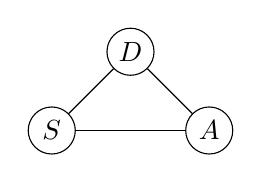
\begin{tikzpicture}
            \tikzstyle{vertex}=[circle,fill=none,draw=black,minimum size=17pt,inner sep=0pt]
\node[vertex] (S) at (0,0) {$S$};
\node[vertex] (A) at (2,0) {$A$};
\node[vertex] (D) at (1,1) {$D$};
\path (S) edge (D);
\path (D) edge (A);
\path (S) edge (A);
            \end{tikzpicture}
        \caption{$\model \in \modelsunconfedge$}
        \label{fig:no-cf-edge}
\end{subfigure}
     \begin{subfigure}{0.32\linewidth}
     \centering
            \begin{tikzpicture}
            \tikzstyle{vertex}=[circle,fill=none,draw=black,minimum size=17pt,inner sep=0pt]
\node[vertex] (S) at (0,0) {$S$};
\node[vertex] (A) at (2,0) {$A$};
\node[vertex] (D) at (1,1) {$D$};
%\node[vertex] (S') at (1,-0.5) {$S'$};
\path (S) edge (D);
\path (D) edge (A);
\path[bidirected] (D) edge[bend left=60] (A);
\path (S) edge (A);
%\path (S) edge (S'); 
% \path (S) edge node[near start, below] {=} (S');
% \draw[->, line width=0.3mm]  (S)--(D);
% \draw[->, line width=0.3mm]  (D)--(A);
% \draw[->, line width=0.3mm]  (S)--(A);
% \draw[<->, line width=0.3mm]  (D)--(A);
            \end{tikzpicture}
        \caption{$\model \in \modelsedgerelax$} 
        \label{fig:cf-edge}
        \end{subfigure}
         \begin{subfigure}{0.32\linewidth}
     \centering
            \begin{tikzpicture}
            \tikzstyle{vertex}=[circle,fill=none,draw=black,minimum size=17pt,inner sep=0pt]
\node[vertex] (S) at (0,0) {$S$};
\node[vertex] (A) at (2,0) {$A$};
\node[vertex] (D) at (1,1) {$D$};
%\node[vertex] (S') at (1,-0.5) {$S'$};
\path (S) edge (D);
\path (D) edge (A);
\path[bidirected] (D) edge[bend left=60] (A);
%\path (S) edge (A);
%\path (S) edge (S'); 
% \path (S) edge node[near start, below] {=} (S');
% \draw[->, line width=0.3mm]  (S)--(D);
% \draw[->, line width=0.3mm]  (D)--(A);
% \draw[->, line width=0.3mm]  (S)--(A);
% \draw[<->, line width=0.3mm]  (D)--(A);
            \end{tikzpicture}
        \caption{$\model \in \nullgraph$ and $\model \in \modeliv$} 
        \label{fig:cf-edge-iv}
        \end{subfigure}
        \caption{Causal graphs, $\cg{\model}$, assumed in various model classes.}
\end{figure*}

% \begin{figure}
%      \centering
%             \begin{tikzpicture}
%             \tikzstyle{vertex}=[circle,fill=none,draw=black,minimum size=17pt,inner sep=0pt]
% \node[vertex] (Z) at (0,0) {$Z$};
% \node[vertex] (Y) at (3,0) {$Y$};
% \node[vertex] (X) at (1.5,0) {$X$};
% %\node[vertex] (S') at (1,-0.5) {$S'$};
% \path (Z) edge (X);
% \path (X) edge (Y);
% \path[bidirected] (X) edge[bend left=60] (Y);
% %\path[red] (S') edge (A);
% %\path (S) edge (S'); 
%  %\path (S) edge node[near start, below] {=} (S');
% % \draw[->, line width=0.3mm]  (S)--(D);
% % \draw[->, line width=0.3mm]  (D)--(A);
% % \draw[->, line width=0.3mm]  (S)--(A);
% % \draw[<->, line width=0.3mm]  (D)--(A);
%             \end{tikzpicture}
%         \caption{Causal graph of $M \in \modeliv$} 
%         \label{fig:iv}
%         \end{figure}

% LLM-based agents integrate the capabilities of language models with reasoning, planning, memory retention, and interaction with external tools~\cite{qin2024toolllm,code-generatingLLMCHI23}.
We propose using LLM-based agents to facilitate the interactive construction of harmonization pipelines through natural language and visual interfaces. We aim to simplify the harmonization process and empower domain experts to harmonize their own data~effectively.

Our approach has three main aspects -- \textit{harmonization primitives}, \textit{harmonization agents}, and \textit{human-agent interaction}, as illustrated in Figure~\ref{fig:system-diagram}. 
The system should support two-way interaction between the \textit{users} and the \textit{harmonization agents}. While the former drives the system and defines the tasks to be performed, the latter aims to automate most data harmonization tasks, leaving only key decisions that need external context to users.
By capturing user-agent interactions and the derived computational pipelines, we maintain the provenance of the harmonization process. This supports transparency and reproducibility, making it possible to publish the harmonized data with the pipeline used to derive it.

\myparagraph{Harmonization Primitives}
The bottom of Figure~\ref{fig:system-diagram} illustrates a library of components that we refer to as \textit{data integration primitives}. These are key algorithms or routines that can be developed to solve well-defined data integration tasks such as schema matching, value matching, % function-attribute matching,
and others. Some of these components are lower-level routines that support other higher-level tasks, e.g., column-type annotation may be a component of schema-matching algorithms~\cite{feuer:vldb2024}, and entity resolution and deduplication may be key to performing data standardization~\cite{christophides2020overview}. While the particular set of primitives can be heterogeneous and evolve to support the system capabilities, they have in common that they need to be \textit{composable} and can be invoked by both user and AI agents.

\textit{Primitive composability} refers to the ability to combine primitives to create a pipeline: the output of a primitive $p_1$ can be used as input of another primitive $p_2$. For example, \textit{schema matching} primitives can output a list of source-target attribute pairs.
These lists form the input for the \textit{value matching} primitives, which then find equivalences between the values of the source attribute to the target. Finally, the output of value-matching primitives can be used to assemble a \textit{harmonization specification} that describes the transformation of source tables $T_i$ into a target output table $T_{target}$.
% 
In short, primitive composability enables the creation of data harmonization pipelines by allowing the chaining of operations that take source tables as input and produce harmonized data as output.

\myparagraph{Data Harmonization Agents}
The harmonization agent fulfills user requests by synthesizing pipelines that perform the requested harmonization task. 
First, it decomposes the problem in a sequence of actions. These actions can be of multiple types, including execution of existing integration primitives (tool calling) or execution of code generated on-demand. 
To decide on what action to take, the harmonization agent leverages an LLM, which is provided with descriptions of the task and integration primitives available for use. 
The LLM then returns an action (e.g., a code snippet) that can be executed in a runtime environment (e.g., a Python kernel). The action output is then fed back into the LLM, which decides if it needs to execute additional actions or if the task is completed.
This loop executes until the task is deemed complete (see Figure~\ref{fig:agent-loop}).
% As illustrated in Figure~\ref{fig:agent-loop}, this loop executes until the task is deemed complete 

The main loop is orchestrated by a driver code that takes inputs from the user (i.e., prompts) that describe the task to be performed. 
This driver is also responsible for (1) communicating with users to request inputs (e.g., when the LLM asks for task clarification or user preferences) and (2) managing the state (memory) of the agent. For example, it can also track and store the history of actions and user interactions in a \textit{Provenance DB}.
This data can support decisions about future actions, and transparency, and be used to generate harmonization \textit{specifications} or scripts to reproduce the results.

Given the complexity of harmonization tasks, it is crucial to have high-level primitives available as building blocks for the pipeline.
This allows encoding prior knowledge and using efficient algorithms known to be effective for a specific task.
These primitives encompass algorithms for tasks such as schema matching, entity resolution, and value mapping. Of course, primitives can go beyond hard-coded functions that implement deterministic algorithms. For instance, they can be workflows that use LLMs to perform specific tasks such as in \cite{liu2024magneto} or they could generate code on demand (e.g., to extract data from or to transform attribute values~\cite{autoformula2024}). 


\myparagraph{Human-Agent Interaction}
A central component of our system architecture is the user-agent interaction. We argue that systems must go beyond text-based conversational interactions: they need to support rich visual data representations and should allow interactions that help users reason about the answers produced by the agent and refine the task definition as well as the pipelines derived by the agent. In complex tasks such as harmonization, this is necessary since many decisions needed to complete the task (e.g., whether two terms represent the same concept) are difficult even for domain experts and may require external knowledge, such as the context in which data was collected.

In this paper, we focus on interactions based on natural language via a chatbot interface. However, it should be possible to implement even more intuitive and efficient graphical interfaces that combine natural language with point-and-click components. For example, as done in interactive AutoML tools~\cite{santos2019visus}, the system may guide the user through the harmonization process, recommend the available actions, track progress, and provide data visualizations to help the user better make sense of the data. This may help prevent common issues in natural language such as ambiguity~\cite{esfandiarpoor2024followup}.

\vspace{-.75em}
\section{System Prototype \& Use Case} \label{sec:prototype}

\myparagraph{The primitives library}
% We used the data harmonization primitives provided by \texttt{bdi-kit} \cite{bdi-kit-github}, an open-source Python library. 
We used data harmonization primitives from \texttt{bdi-kit} \cite{bdi-kit-github}, an open-source Python library that we designed with the explicit goal of composability.
%We implemented the data harmonization primitives library in Python and released it as the Python library that we call \texttt{bdi-kit} \cite{bdi-kit-github}. 
Currently, it includes implementations of multiple \textit{schema matching} and \textit{value matching} algorithms using a composable API. It includes several classic algorithms from Koutras et al.~\cite{koutras2021valentine} and language model-based algorithms such as the ones presented in~\cite{liu2024enhancing} and \cite{liu2024magneto}. Most functions take as input a \texttt{source} parameter that represents the user's input DataFrame and returns the output formatted as another DataFrame. The \texttt{target} parameter can either be a string representing a target standard schema (e.g., \texttt{`gdc'}) or a target DataFrame, this allows switching between the two tasks described in Examples~\ref{example1} and ~\ref{example2}. Figure~\ref{fig:bdi-kit} shows a subset of functions relevant to this paper.

\begin{figure}[t]
% \vspace{-1.25em}
\centering
\begin{tcolorbox}[colback=black!2.5!white,colframe=black!85!black,boxrule=0.25mm,boxsep=4pt,left=0pt,right=0pt,top=0pt,bottom=0pt]

    \footnotesize
    
    \texttt{\textbf{match\_schema}(source, target, method, ...)} \\
    Maps the schema of a source table to a target schema (table or predefined standard like \texttt{gdc}) using a specified method.
    \vspace{.5em}
    
    
    \texttt{\textbf{top\_matches}(source, column, target, top\_k, method, ...)} \\
    Finds the top-\texttt{k} matches between a source column and columns of a target schema.
    \vspace{.5em}
    
    
    \texttt{\textbf{match\_values}(source, target, column\_mapping, method, ...)} \\
    Matches values between columns of a source and a target using a specified method, returning one or more result tables.
    \vspace{.5em}
    
    
    % \texttt{\textbf{top\_value\_matches}(source, target, column\_mapping, top\_k,...)} \\ %  method, 
    % Finds the top-\texttt{k} value matches between columns in a source and target.
    % \vspace{.5em}
    
    
    % \texttt{\textbf{view\_value\_matches}(matches, edit = False)} \\
    % Displays value match results in a table format, with optional editing.
    % \vspace{.5em}

    
    % \texttt{\textbf{preview\_domain}(dataset, column, limit = None) → DataFrame} \\
    % Previews unique values and descriptions in a specified column of a dataset.
    % \vspace{.5em}

    
    % \texttt{\textbf{merge\_mappings}(mappings, user\_mappings = None) → List} \\
    % Combines computed and user-provided mappings into a plan for data transformation.
    % \vspace{.5em}

    
    \texttt{\textbf{materialize\_mapping}(input\_table, mapping\_spec) → DataFrame} \\
    Transforms a source table into a new table using a mapping specification.
    % 
    % \texttt{create\_mapper(input) → ValueMapper} \\
    % Creates a mapper object for transforming column values based on the input type. \\
    
    % \texttt{MappingSpecLike} \\
    % Defines mappings between source and target columns, including optional value transformations. \\
\end{tcolorbox}
% \vspace{-1.5em}
\caption{A subset of functions available in the \texttt{bdi-kit} API.}
% \vspace{-1.5em}
\label{fig:bdi-kit}
\end{figure}

\myparagraph{The data harmonization agent} We implemented \systemname, a system prototype that uses the data integration primitives from Figure~\ref{fig:bdi-kit} and interacts with users via a text-based chat box. Implementing an agent entails writing carefully crafted function and task descriptions that are combined to assemble system prompts fed to the LLMs. For our prototype, we implemented tool wrappers for each of the \texttt{bdi-kit} functions, along with descriptions of when each should be used. We also provide general descriptions of the data harmonization steps, when the LLM should request help from the user, and output formatting instructions.

To implement the tool calling functionality and the user interface, we used the Archytas~\cite{archytas} library, an open-source tool for building AI agents based on the ReAct framework~\cite{yao2022react}, and Beaker~\cite{beaker}, a contextually-aware notebook system that supports the development of chatbot user interfaces. This allows us to implement features that facilitate interaction, such as rendering markdown-formatted outputs in the browser, displaying the reasoning steps taken by the agent, collecting user inputs, and feeding them back to the agent.

%\myparagraph{Use case: harmonization with the GDC standard} % previous title
\myparagraph{Human-agent interaction: The GDC use case}
To demonstrate the ability to produce good data harmonization plans, we present a use case that harmonizes a dataset from Dou et al.~\cite{dou2020proteogenomic} (described in Example~\ref{example1}) with the GDC standard. 
% Below we provide an example of interaction with the chatbot agent.
Below, we show message exchanges between the user ({\scriptsize \faUser}) and the agent ({\scriptsize \faRobot}), along with explanations of the actions taken by the agent to answer user queries.

The user starts by requesting the system to load a CSV file that contains the attributes of interest:
% \vbox{
% \vspace{-.5em}
\chatboxUser{
Load the file dou.csv as a dataframe and subset it to the following columns: Country, Histologic\_Grade\_FIGO, Histologic\_type, FIGO\_stage, BMI, Age, Race, Ethnicity, Gender, Tumor\_Focality, Tumor\_Size\_cm.
}
% \vspace{-1em}
\chatboxAgent{
The file 'dou.csv' has been successfully loaded and subsetted to the specified columns: Country, Histologic\_Grade\_FIGO, Histologic\_type, FIGO\_stage, BMI, Age, Race, Ethnicity, Gender, Tumor\_Focality, Tumor\_Size\_cm.\\
Outputs:\\
{\color{gray}[...data frame displayed here...]}
}
\vspace{-.5em}
% }
\noindent Responding to this prompt, the agent automatically (1) generates Python code using the Pandas library that loads and selects the requested columns and (2) executes the generated code to load the CSV file into memory. This example illustrates the capability of \textit{on-demand code generation} to accomplish a requested task.

Next, the user requests the system to perform schema matching between the table loaded and the attributes from the GDC standard:

% \vspace{-.5em}
\chatboxUser{
Please match this to the GDC schema using the `ct\_learning' method, and fix any results that don't look correct.
}
% \vspace{-.5em}

\noindent
As shown in Figure~\ref{fig:sequence-diagram}, the system interacts with an LLM multiple times to answer this request. First, it sends the initial user's prompt to the LLM, which recognizes that the function \texttt{match\_schema} is adequate to solve the request, and thus returns a tool calling instruction containing the \texttt{match\_schema} function name along with the needed parameters. Note that the LLM parses the user's query, and recognizes that \texttt{gdc} must be used as the target schema and \texttt{ct\_learning} refers to the argument \texttt{method} of \texttt{match\_schema()}. 
% 
After receiving the tool calling instruction as output, the system then executes the primitive function requested by the LLM, collects the list of column matches returned, and passes it back to the LLM in a follow-up prompt. 

After analyzing the column match results received in the follow-up prompt, the LLM detects a mapping mistake for the column \texttt{Histologic\_type}, which is wrongly mapped to \texttt{roots}. To fix the error, the LLM triggers a tool calling instruction that uses the primitive function \texttt{top\_matches} to find the top~10 alternative candidates for \texttt{Histologic\_type}. After receiving the results, it analyzes the results and suggests using \texttt{primary\_diagnosis} as a correction to the user (who agrees) as seen in the following messages:

\vbox{
% \vspace{-.5em}
\chatboxAgent{The current mapping for `Histologic\_type' is `roots', which seems incorrect. The top alternatives are:\\
- history\_of\_tumor\_type\\
- primary\_diagnosis\\
- sample\_type\\
I suggest using `primary\_diagnosis'. Do you agree with this choice?
}
% \vspace{-1em}
\chatboxUser{yes}
}
\vspace{-.5em}
\noindent 
As a final response to the task, the agent shows a table of column mappings as output, where the ``\texttt{Source Column}'' contains columns from the source table (\texttt{dou.csv}), ``\texttt{Target Column}'' contains a column match from the GDC standard, and ``\texttt{Corrected?}'' indicates whether the LLM has corrected the original \texttt{bdi-kit} match.

\vspace{-.25em}
\chatboxAgent{
Result:\\

% \scriptsize
\vspace{-0.25em}
\hspace{-0.25cm}
\begin{tabular}{lll}
\textbf{Source Column} & \textbf{Target Column} & \textbf{Corrected?} \\
Country & country\_of\_birth & No \\
Histologic\_Grade\_FIGO & tumor\_grade & No \\
Histologic\_type & primary\_diagnosis & Yes, from ``roots'' \\
FIGO\_stage & figo\_stage & No \\
BMI & bmi & No \\
Age & age\_at\_onset & No \\
Race & race & No \\
Ethnicity & ethnicity & No \\
Gender & gender & No \\
Tumor\_Focality & tumor\_focality & No \\
Tumor\_Size\_cm & tumor\_depth\_measurement & No \\
\end{tabular}
}
% }

Since the user is a domain expert who knows the GDC standard and knows that there may be better options for \texttt{Tumor\_Size\_cm}, it asks the system to find an alternative match. The system then updates the previous list with a more appropriate match found using the \texttt{top\_matches} function. This interaction is shown next:

\vbox{
% \vspace{-.25em}
\chatboxUser{
Find alternative mappings for Tumor\_Size\_cm.
}
% \vspace{-1em}
\chatboxAgent{Result:\\

\scriptsize
\vspace{-0.25em}
\hspace{-0.25cm}
\begin{tabular}{lll}
    \textbf{Source Column} & \textbf{Target Column} & \textbf{Corrected?} \\ 
    {\color{gray}[...]} & {\color{gray}[...]} & {\color{gray}[...]} \\
    % Country & country\_of\_birth & No \\ 
    % Histologic\_Grade\_FIGO & tumor\_grade & No \\ 
    % Histologic\_type & primary\_diagnosis & Yes, from "roots" \\ 
    % FIGO\_stage & figo\_stage & No \\ 
    % BMI & bmi & No \\ 
    % Age & age\_at\_onset & No \\ 
    % Race & race & No \\ 
    % Ethnicity & ethnicity & No \\ 
    % Gender & gender & No \\ 
    Tumor\_Focality & tumor\_focality & No \\ 
    % Tumor\_Size\_cm & tumor\_largest\_dimension\_diameter & Yes, from "tumor\_depth\_measurement" \\ 
    Tumor\_Size\_cm & tumor\_largest\_dimension\_diameter & Yes, from "tumor\_depth... \\ 
\end{tabular}
}
} %\vbox

% --------------
% Value mappings
% --------------

After finding correct matches for all source columns, the next step is to find value mappings for each column match. The following prompt requests the agent to find such mappings:

% \vspace{-0.75em}
% \vbox{
\chatboxUser{\raggedright Find value mappings for the columns Country, Histologic\_Grade\_FIGO, Histologic\_type, FIGO\_stage, Race, Ethnicity, Gender, Tumor\_Focality. If there are any errors in the mappings, please provide suggestions.
}
% \vspace{-0.75em}
\noindent
As in the previous prompts, finding value mappings requires multiple LLM interactions. First, the LLM triggers one function call of \texttt{match\_values()} for each of the source-target column pairs using the default value matching method \texttt{tfidf}  (an efficient algorithm that chooses matches based on the tf-idf similarity over character n-grams). After receiving the value matches, the LLM evaluates if they are correct, and fixes the entries that contain errors. To do so, it calls another function to discover the list of acceptable values in a GDC attribute and picks the correct one. A snippet of the result is shown next (we omit part of the output due to lack of space):
%in the box below:

\vspace{-0.5em}
\chatboxAgent{\scriptsize
{\color{gray}[...]}\\

\vspace{-0.5em}
\textbf{Histologic\_Grade\_FIGO → tumor\_grade}\\

\vspace{-0.5em}
\hspace{-0.25cm}
\begin{tabular}{lll}
    \textbf{Source Value} & \textbf{Target Value} & \textbf{Corrected?} \\ 
    FIGO grade 1 & G1 & Yes, from "Low Grade" \\ 
    FIGO grade 2 & G2 & Yes, from "Low Grade" \\ 
    FIGO grade 3 & G3 & Yes, from "Low Grade" \\ 
\end{tabular}\\

{\color{gray}[...]}\\

\vspace{-0.25em}
\textbf{FIGO\_stage → figo\_stage}\\

\vspace{-0.25em}
\hspace{-0.25cm}
\begin{tabular}{lll}
    \textbf{Source Value} & \textbf{Target Value} & \textbf{Corrected?} \\ 
    IIIC2 & Stage IIIC2 & No \\ 
    IIIC1 & Stage IIIC1 & No \\ 
    IVB & Stage IVB & No \\ 
    IIIB & Stage IIIB & No \\ 
    IIIA & Stage IIIA & No \\ 
    II & Stage II & Yes, from "Stage III" \\ 
\end{tabular}\\

\vspace{-0.25em}
{\color{gray}[...]}
}
% \vspace{-0.5em}
% }

\noindent
This example illustrates the ability of the LLM to detect and correct errors automatically without the user's intervention. As an example, it corrects the match $\langle\texttt{II}, \texttt{Stage III}\rangle$ to $\langle\texttt{II}, \texttt{Stage II}\rangle$. This showcases how we can leverage existing fast algorithms to perform most of the work while leveraging LLMs as an evaluator that can detect and fix mistakes only when needed.

% ------------------
% Materialize schema
% ------------------

The final step is generating a harmonized table. The boxes below show the user prompt as well as the agent response:

\vbox{
% \vspace{-0.25em}
\chatboxUser{Please create a final harmonized table based on the discovered column and value mappings and save it at "dou\_harmonized.csv".}
% \vspace{-1em}
\chatboxAgent{The harmonized table has been successfully created and saved as `dou\_harmonized.csv'.}
% \vspace{-0.25em}
}
\noindent
In this example, the agent uses \texttt{materialize\_mapping} to generate a table and save file \texttt{`dou\_harmonized.csv'}. The LLM  first creates a declarative mapping specification according to the bdi-kit's format used to describe a harmonization plan. Figure~\ref{fig:mapping-spec} shows a snippet of the generated harmonization plan, which includes a declarative specification of the mappings to be performed written in JSON. In this example, we only show dictionary-based transformations that map source values into target values. However, bdi-kit's also supports other types of transformations, such as custom mappings that take as input a custom Python function (or lambda).
This can potentially be used along with the on-demand code generation.

The main advantage of using a declarative language to describe harmonization plans is that it enables reproducibility: once a plan is created, users can feed the plan along with the source data into \texttt{materialize\_mapping} function to recreate the harmonized data. This does not require re-running any LLM-based interactions, since all transformations are encoded in the harmonization plan.

% This is a hack to remove the syntax highlighting error in the minted box below
\AtBeginEnvironment{minted}{\renewcommand{\fcolorbox}[4][]{#4}}
\begin{figure}[h]
\vspace{-.75em}
\begin{tcolorbox}[colback=black!2.5!white,colframe=black!85!black,boxrule=0.25mm,boxsep=4pt,left=0pt,right=0pt,top=0pt,bottom=0pt]
\begin{minted}[fontsize=\scriptsize]{json}
[ 
 [...]
 { "source": "Country",
   "target": "country_of_birth",
   "matches": [ ["United States", "United States"],
                ["Poland", "Poland"],
                ["Ukraine", "Ukraine"] ] },
 { "source": "Histologic_Grade_FIGO",
   "target": "tumor_grade",
   "matches": [ ["FIGO grade 1", "G1"],
                ["FIGO grade 2", "G2"],
                ["FIGO grade 3", "G3"] ] },
 [...]
]
\end{minted}
\end{tcolorbox}
\vspace{-1.25em}
\caption{A snippet from the mapping specification generated that is passed to \texttt{materialize\_mapping()} function.}
\label{fig:mapping-spec}
\end{figure}

\section{Research Opportunities}
\label{sec:research-agenda}

\systemname shows the potential of LLM-based agents to orchestrate actions, evaluate function outputs, detect errors, and generate additional needed functions. However, there are still open research opportunities to expand the system's capabilities.
Below we outline some of the immediate steps towards these opportunities.


% ----------------------------------------------------
\myparagraph{Agent Evaluation \& Benchmarks} 
Most existing evaluation benchmarks are focused on isolated tasks, such as schema matching or entity linking~\cite{koutras2021valentine, liu2024magneto, wang2021machamp}. 
However, agentic systems create a need for end-to-end evaluation benchmarks and metrics to measure progress effectively. Recently, researchers have started developing benchmarks for evaluating agents in various tasks, including data analysis and ML engineering~\cite{chan2024mle, hu2024infiagent, zhang2024benchmarking, huang2024mlagentbench}. 
The data management community should follow this lead and create benchmarks tailored for data integration, ensuring that LLMs improve in these areas.


\myparagraph{Data Integration Primitives}
\label{sec:proposed-primitives}
Some features, such as \emph{uncertainty} quantification and \emph{explanations}, should be exposed by the primitives to guide decision-making~\cite{uncertainty2009}.
Uncertainty in data integration arises from factors like ambiguous schema mappings and data values~\cite{WangHM2018}. \systemname tackles this by exposing similarity scores through its primitives. For example, a value matcher can return similarity scores, so the agent can strategically trigger complementary primitives (e.g., value mapping) for deeper analysis. A key challenge is conveying the meaning of uncertainty measures from diverse primitive mechanisms to both LLMs and end users, and instructing LLMs on how to use and act on them properly~\cite{dagstuhl2029explanation}.

On the same note, LLMs often lack transparency~\cite{pmlr-v235-huang24x}, so primitives must provide \textit{interpretable explanations} to promote user trust. Primitives should offer clear usage documentation and expose their decision rationale. For instance, a matching algorithm description should document whether its similarity scores derive from syntactic similarity, semantic embeddings, or value distribution analysis. LLMs can also explain their decisions based on domain knowledge and primitive instructions, helping users better understand why a particular path was chosen~\cite{explainability2024,TableMeetsLLM2024}. A key opportunity is training agents to discern when to rely on LLM explanations, apply alternative strategies, or engage with the user directly.

Mapping data between schemata involves resolving entities and transforming data~\cite{dataexchange2018}. LLM-based methods have proven helpful in entity resolution~\cite{narayan-vldb2022, fan2024cost}, generating or finding transformations functions~\cite{zdnet-github-copilot, trummer2022codexdb,autotables2023, autoformula2024, dtt2024, SheetAgent2024}, and evaluating LLM performance on such tasks~\cite{ma2024spreadsheetbench}.
However, integrating these methods into agent-based systems requires consistency across diverse data models and alignment with broader agent goals.
Also, we need methods that allow agents to identify and recommend appropriate attribute transformations and suitable functions for a given input dataset. This is especially in challenging cases such as table restructuring or non-standard formats~\cite{autotables2023}.
Another immediate step is to curate a library of transformation functions specialized in data transformation tasks that agentic systems can readily reuse.


\myparagraph{Robustness and Reliability}
LLMs have shown inconsistency across various scenarios (e.g., as text summarization evaluators~\cite{stureborg2024large}), often producing varying results when executed multiple times~\cite{barrie2024prompt}. This variability can undermine reproducibility and reliability, particularly in critical applications where consistent mappings or transformations are crucial. In our experiments, we observed that while the LLM typically identified and fixed incorrect mappings, it occasionally failed to do so (even when provided with the same prompts).

Handling large and complex tables with many attributes poses additional challenges, as these can lead to long chat histories that exceed the LLM context window. When this occurs, the LLM may lose access to earlier relevant information, thereby affecting the robustness. While approaches have been proposed to mitigate context window limitations (e.g., \cite{jin2024llm} \cite{ma2024megalodon}), 
it is not clear if they address the issues in agent systems. 
Equipping agents with access to read and store data in external databases (such as the Provenance DB discussed in Section ~\ref{sec:agentic-data-harmonization}) may be an effective solution to this issue.

\myparagraph{User-Agent Interaction} To improve usability, agentic systems must go beyond natural language (NL) interfaces. While NL is flexible, it is also often ambiguous and may lead to under-specified task descriptions~\cite{zhang2023clarify}. 
Since the same task can be expressed in multiple unpredictable ways, a mismatch between the user task descriptions and agent prompt specifications may occur. Therefore, detecting when clarifications are needed may help increase overall success~\cite{zhang2023clarify}.
These issues could also be potentially addressed by action-oriented UIs that recommend actions linked to predefined prompts. Moreover, using rich visual representations may be more effective at conveying information to the user.

\myparagraph{Provenance-Aware Agents} 
Provenance collection systems have demonstrated promising results in data science pipelines ~\cite{rupprechtVLDB2020,chapmanCapturing2020}.
In data harmonization pipelines, we can track all interactions that contribute to obtaining a specific value mapping. For example, we could record all user-agent and agent-primitive interactions involved in determining the mapping of ``\texttt{FIGO grade 1}'' to ``\texttt{G1}'' (see Figure \ref{fig:mapping-spec}). 
This would allow tracing the lineage of all values in the output data. Moreover, this information could potentially be used to learn user preferences that reduce the need for user interactions.
% Such systems not only enhance transparency but also reduce the need for user interactions, particularly for new practitioners. 
By learning from provenance and pipelines accumulated over time, a system could further streamline the harmonization process by automating all steps and presenting final results directly to users.
% For instance, a provenance system could streamline the harmonization process by bypassing intermediate steps and presenting final results directly to new users.


\myparagraph{Data Harmonization Pipelines} 
In our system, data harmonization is expressed as a pipeline where multiple primitives (predefined, user-defined, or agent-defined) are interconnected through their inputs and outputs to produce the final harmonized dataset. 
% The pipeline can have various objectives, such as creating a dataset with a desired minimum number of rows, returning a sample result in a few seconds, or generating a high-quality dataset based on a chosen quality metric. 
The pipeline can have various objectives, such as maximining the number of correct column matches and value matches, minimizing the number of interactions with users, or minimizing the computational costs (e.g., runtime or LLM calls).
Achieving these objectives represents an optimization problem, requiring the system to navigate a complex search space and balance multiple objectives to determine an optimal sequence of operations.

Recent work has explored large search spaces for building end-to-end pipelines for various tasks~\cite{lopez2023alphad3m,substrat2022,autopipeline2012vldb,volcanoVLDB2021}. AutoML provides a relevant example where the focus is usually on model quality, and the system selects the best algorithms, features, and hyperparameters~\cite{lopez2023alphad3m}. Pipeline generation for data harmonization can build on such advancements. 
%Still, the task is further complicated by the input data's inherent uncertainty and variability.
An immediate step is building optimizers that measure and balance multiple objectives like harmonization success and computational costs.
Also, our system integrates human-in-the-loop interactions to iteratively refine pipelines based on user feedback and domain expertise. 
An open challenge is determining how to effectively balance automation and human input~\cite{human-in-the-loopdataintegration2017}.

\myparagraph{Acknowledgments}
This work was supported by NSF awards IIS-2106888 and OAC-2411221, and the DARPA
% Automating Scientific Knowledge Extraction and Modeling (ASKEM) program,
ASKEM program
Agreement No. HR0011262087. The views, opinions, and findings expressed are those of the authors and should not be interpreted as representing the official views or policies of the DARPA, the U.S. Government, or NSF.


\bibliographystyle{ACM-Reference-Format}
\bibliography{main}
% \balance

\end{document}
